%%
% This is an Overleaf template for presentations
% using the TUM Corporate Desing https://www.tum.de/cd
%
% For further details on how to use the template, take a look at our
% GitLab repository and browse through our test documents
% https://gitlab.lrz.de/latex4ei/tum-templates.
%
% The tumbeamer class is based on the beamer class.
% If you need further customization please consult the beamer class guide
% https://ctan.org/pkg/beamer.
% Additional class options are passed down to the base class.
%
% If you encounter any bugs or undesired behaviour, please raise an issue
% in our GitLab repository
% https://gitlab.lrz.de/latex4ei/tum-templates/issues
% and provide a description and minimal working example of your problem.
%%


\documentclass[
  english,            % define the document language (english, german)
  aspectratio=169,    % define the aspect ratio (169, 43)
  % handout=2on1,       % create handout with multiple slides (2on1, 4on1)
  % partpage=false,     % insert page at beginning of parts (true, false)
  % sectionpage=true,   % insert page at beginning of sections (true, false)
]{tumbeamer}

%\setbeameroption{hide notes} % Only slides
\setbeameroption{show only notes} % Only notes
%\setbeameroption{show notes on second screen=right} % Both

% load additional packages
\usepackage{booktabs}
\usepackage{graphicx}
\graphicspath{ {./images/} }

% presentation metadata
\title{Compressed Sensing}
\subtitle{Seminar of Mathematics in Data Science \newline (Prof. Dr. Massimo Fornasier, PD Dr. Peter Massopust) }
\author{Oleksii Davydenko}

\institute{\theChairName\\\theDepartmentName\\\theUniversityName}
\date[30/06/2021]{June 30\textsuperscript{th}, 2021}

\footline{\insertauthor~|~\insertshorttitle~|~\insertshortdate}


% macro to configure the style of the presentation
\TUMbeamersetup{
  title page = TUM tower,         % style of the title page
  part page = TUM toc,            % style of part pages
  section page = TUM toc,         % style of section pages
  content page = TUM more space,  % style of normal content pages
  tower scale = 0.7,              % scaling factor of TUM tower (if used)
  headline = TUM threeliner,      % which variation of headline to use
  footline = TUM default,         % which variation of footline to use
  % configure on which pages headlines and footlines should be printed
  headline on = {title page},
  footline on = {every page, title page=false},
}

% available frame styles for title page, part page, and section page:
% TUM default, TUM tower, TUM centered,
% TUM blue default, TUM blue tower, TUM blue centered,
% TUM shaded default, TUM shaded tower, TUM shaded centered,
% TUM flags
%
% additional frame styles for part page and section page:
% TUM toc
%
% available frame styles for content pages:
% TUM default, TUM more space
%
% available headline options:
% TUM empty, TUM oneliner, TUM twoliner, TUM threeliner, TUM logothreeliner
%
% available footline options:
% TUM empty, TUM default, TUM infoline


\begin{document}

\maketitle

\section{Problem Statement}

\begin{frame}{Problem Statement}{}
  \textbf{Goal}: Recover a (sparse) signal from its reduced representation (measure).
  
  \bigskip Fundamental theorem of linear algebra: in order to effectively reconstruct a signal we need a sequence of measurements that is at least as long as the original signal.
  
  \bigskip Assume sparsity -> recover signal from "incomplete" measures!
  
  \bigskip This applies primarily in situations when repeated measures are costly or harmful (like in the case of magnetic resonance imaging) or when measures are naturally sparse (like radar scans).
  
  \note[item]{A question of interest is whether there is a good way of obtaining the compressed version of the signal directly, without taking many measurements of it. Compressed sensing is relying on taking a small amount of linear and non-adaptive measurements. Interestingly enough, all provably good measurement matrices happen to be random matrices. These include the Gaussian, Bernoulli and partial random Fourier matrices.}
\end{frame}

\begin{frame}{Applications}{on naturally sparse data}
  \begin{columns}
      \begin{column}{.5\linewidth}\centering
          \begin{itemize}
              \item Magnetic Resonance Imaging (MRI)
              \item Radar data
              \note[item]{In radar imaging, only a small amount of targets is monitored at the same time, so sparsity becomes a very realistic assumption. Standard methods for radar imaging actually use the sparsity assumption as well, but only at the very end of the signal processing procedure in order to clean up the noise in the resulting image. Using sparsity from the very beginning by using compressive sensing methods is therefore a natural approach.}
              \item Wireless communication
              \item Astronomical signal and image processing
              \item Camera design and imaging
              \item Collaborative filtering
              \item Matrix completion
              \note[item]{Collaborative filtering and matrix completion are actively used in recommender systems}
          \end{itemize}
          \bigskip \bigskip \bigskip Image sources: \href{https://radiology.ca/article/how-does-mri-help-diagnose-ms}{[1]} and \href{http://research.atmos.ucla.edu/weather/C227/Documents/tmp/basic_wxradar/print.php.htm}{[2]}
      \end{column}
      \begin{column}{.5\linewidth}\centering
        \par 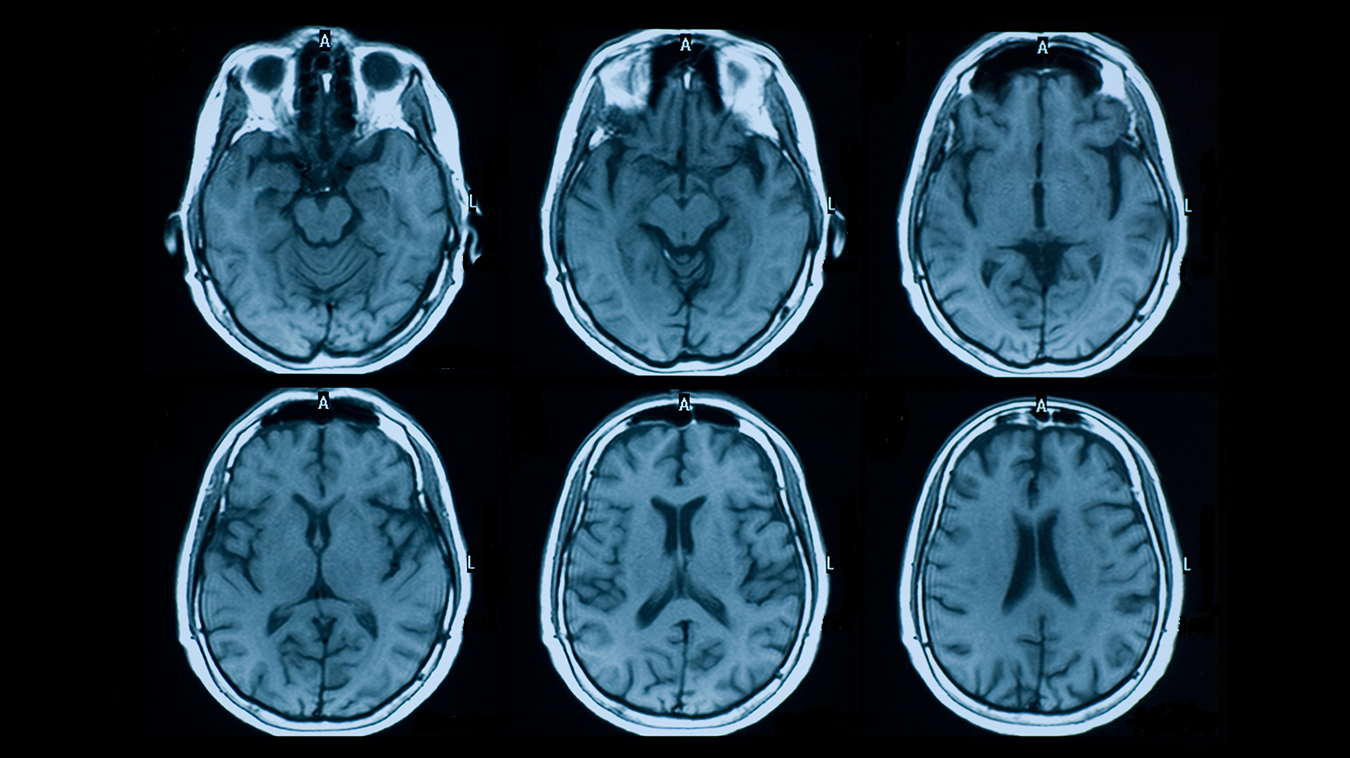
\includegraphics[width=\linewidth/2]{MRI-Brain.jpg}
        \par 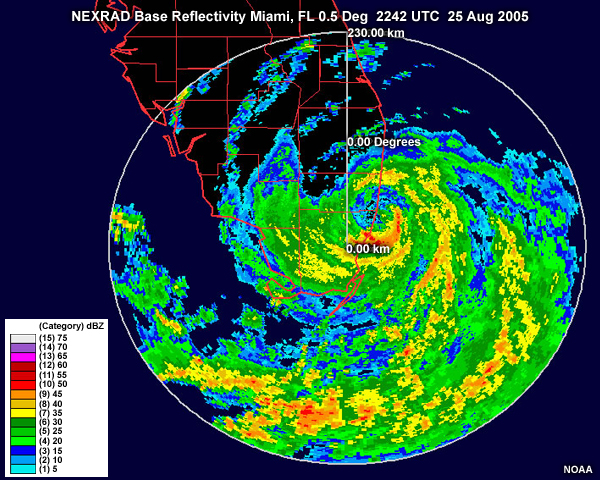
\includegraphics[width=\linewidth/2]{images/katrina_radar_fla.jpg}
      \end{column}
  \end{columns}
\end{frame}

\section{Mathematical Notation}

\begin{frame}{Why $l_1$ optimization?}
Our signal transformation process can be described as $y = Ax$, where $x \in \mathbb{C}^N$, $A \in \mathbb{C}^{m \times N}$ - the \textit{measurement matrix}, $y \in \mathbb{C}^m$ - \textit{measurement vector}. We are especially interested in the case when $m << N$. With the additional assumption that x is k-sparse, restoring it from y becomes realistic. The $l_1$-minimization approach considers the solution of 
\[min \lVert z \rVert _1 \text{ subject to } Az = y\]
which is a convex problem and can be seen as a convex relaxation of
\[min \lVert z \rVert _0 \text{ subject to } Az = y\]
$l_1$-minimization tends to promote sparse solutions.
\end{frame}

\begin{frame}{Sparse Vectors}
We denote the support of the vector $x$ as $supp(x) = \{j : x_j \neq 0\}$, and 
\[ \lVert x \rVert_0 := |supp(x)| \]
denotes the "$l_0$-norm" of the vector, even though formally it is not a norm.

Then a vector x is called \textit{k-sparse} if $\lVert x \rVert_0 \leq k$. We can now define the best k-term approximation error of a vector $x \in \mathbb{C}^N$ as
\[ \sigma_k (x)_p = \inf_{z \in \Sigma_k} \lVert x - z \rVert_p, \]
where $\Sigma_k$ is a set of all $k$-sparse vectors
\[\Sigma_k := \{x \in \mathbb{C}^N : \lVert x \rVert_0 \leq k\}. \]
\end{frame}

\begin{frame}{The Null Space Property}
The null space property provides the necessary and sufficient conditions on the reconstruction of signals using the techniques of $l_1$-relaxation.

\bigskip \textbf{Definition 1.} A matrix $A \in \mathbb{C}^{m \times N}$ is said to satisfy the null space property (NSP) of order $k$ with constant $\gamma \in (0, 1)$ if
\[ \lVert \eta_T \rVert_1 \leq \gamma \lVert  \eta_{T^c} \rVert_1 \]
for all sets $T \subset \{1,...,N\}, \#T \leq k$ and for all $\eta \in ker A$.

\bigskip \textbf{Theorem 1.} Let $A \in \mathbb{C}^{m \times N}$ be a matrix that satisfies the NSP of order k with constant $\gamma \in (0, 1)$. Let $x \in \mathbb{C}^N$ and $y = Ax$ and let $x^*$ be a solution of the $l_1$-minimization problem. Then
\[ \lVert x - x^* \rVert_1 \leq \frac{2(1+\gamma)}{1-\gamma} \sigma_k(x)_1 \]
In particular, if x is k-sparse then $x^* = x$.

\end{frame}

\begin{frame}{The Null Space Property}
The null space property provides the necessary and sufficient conditions on the reconstruction of signals using the techniques of $l_1$-relaxation.

\bigskip \textbf{Definition 1.} A matrix $A \in \mathbb{C}^{m \times N}$ is said to satisfy the null space property (NSP) of order $k$ with constant $\gamma \in (0, 1)$ if
\[ \lVert \eta_T \rVert_1 \leq \gamma \lVert  \eta_{T^c} \rVert_1 \]
for all sets $T \subset \{1,...,N\}, \#T \leq k$ and for all $\eta \in ker A$.

\bigskip It is also possible to show that if all k-sparse x can be recovered from $y = Ax$ using $l_1$-minimization the necessarialy $A$ satisfies the NSP of order k with some constant $\gamma \in (0,1)$. This means that NSP is actually equivalent to sparse $l_1$-recovery.
\end{frame}

\begin{frame}{Restricted Isometry Property}

Since the NSP is difficult to show directly, the restricted isometry property (RIP) is used, which is easier to handle and it also implies stability under noise.

\bigskip \textbf{Definition 2.} The restricted isometry constant $\delta_k$ of a matrix $A \in \mathbb{C}^{m \times N}$ is the smallest number such that
\[ (1 - \delta_k) \lVert z \rVert^2_2 \leq \lVert Az \rVert^2_2 \leq (1 + \delta_k) \lVert z \rVert^2_2 ,\]
for all $z \in \Sigma_k$.

A matrix A is said to satisfy the restricted isometry property of order k with constant $\sigma_k$ if $\sigma_k \in (0,1)$. $\sigma_k$ can also be equivalently defined as
\[ \delta_k = \max_{T \subset \{1,...,N\}, \#T \leq k} \lVert A_T^* A_T - I \rVert_{2 \rightarrow 2} ,\]
which means that all column submatrices of A with at most k columns are required to be well-conditioned.
\end{frame}

\begin{frame}{Connection between RIP and NSP}
The RIP implies the NSP as shown in the following lemma.

\bigskip \textbf{Lemma 1.} Assume that $A \in \mathbb{C}^{m \times N}$ satisfies the RIP of order $K = k + h$ with constant $\sigma_k \in (0,1)$. Then A has the NSP of order k with constant $\gamma = \sqrt{\frac{k}{h}\frac{1+\sigma_K}{1-\sigma_K}}$
\end{frame}

\section{$l_1$-minimization Algorithms}

\begin{frame}{Many ways to do $l_1$-optimization}
    \begin{itemize}
        \item Chambolle and Pock's Primal Dual algorithm
        \item Iteratively Reweighted Least Squares (IRLS)
        \item LARS method
        \item Orthogonal Matching Pursuit
        \item CoSaMP
        \item Iterative hard thresholding
    \end{itemize}
\end{frame}

\begin{frame}{Proximal mapping}
For some convex function $G$ the proximal mapping is defined as
\[ P_G(\tau, z) := arg \min_{x \in \mathbb{C}^N} \{\tau G(x) + \frac{1}{2} \lVert x - z \rVert_2^2\} \]
and
\[ F^*(\xi) = sup \{ Re\langle z,\xi \rangle - F(z) : z \in \mathbb{C}^m \} \]
denotes the convex (Fenchel) conjugate of F.
\end{frame}

\begin{frame}{Chambolle and Pock's algorithm}
A goal of the primal dual approach is to solve the optimization problem in the form
\begin{equation}
    \min_{x \in \mathbb{C}^N} F(Ax) + G(x).
\end{equation}
It performs an iteration on the dual variable, the primal variable and an auxiliary primal variable. The initial points are defined as $x^0, \bar{x}^0 = x \in \mathbb{C}^N, \xi^0 \in \mathbb{C}^m$ and parameters $\tau, \sigma > 0, \theta \in [0,1]$, we iteratively compute
\begin{equation}
    \xi^{n+1} := P_{F^*}(\sigma;\xi^n + \sigma A \bar{x}^n),
\end{equation}
\begin{equation}
    x^{n+1} := P_G(\tau; x^n - \tau A^* \xi^{n+1}),
\end{equation}
\begin{equation}
    \bar{x}^{n+1} := x^{n+1} + \theta (x^{n+1} - x^n),
\end{equation}
\end{frame}

\begin{frame}{Chambolle and Pock's algorithm}
This algorithm converges to the saddle point of the primal dual problem, and can be interpreted as a gradient descent method for solving the primal problem, combined with a gradient ascent method to simultaneously solve the dual problem. Its convergence has been proven (see the seminar paper).
\end{frame}

\begin{frame}{Iteratively reweighted least squares (IRLS)}
This iterative algorithm assumes that A satisties the NSP and is guaranteed to reconstruct vectors with the same error estimate as $l_1$-minimization. The algorithm has a guaranteed linear rate of convergence which can even be improved to superlinear rate with a small modification.

Denote $\mathcal{F}(y) = \{x : Ax = y\}$ and $\mathcal{N} = ker A$. Observe that $|t| = \frac{t^2}{|t|}$ for $t \neq 0$. Hence, an $l_1$-minimization can be recasted into a weighted $l_2$-minimization, with the hope that
\[ arg \min_{x \in \mathcal{F}(y)} \sum_{j=1}^N |x_j| \approx arg \min_{x \in \mathcal{F}(y)} \sum_{j=1}^N x_j^2 |x_j^*|^{-1} ,\]
as soon as $x^*$ is the desired $l_1$-norm minimizer. The advantage of the reformulation is that minimizing the smooth function $t^2$ is much easier than minimizing the nonsmooth function $|t|$. However, neither one disposes of $x^*$ a priori (this is the vector we are interested in computing), and we cannot expect that $x_j^* \neq 0$ for all $j = 1,...,N$, since we hope for $k$-sparse solutions.
\end{frame}

\begin{frame}{Iteration}
If we had a good approximation $w_j^n$ of $|(x_j^*)^2 + \epsilon_n^2|^{-1/2} 
\approx |x_j^*|^{-1}$, for some $\epsilon_n > 0$, we could compute
\begin{equation} \label{irls:eq1}
x^{n+1} = arg \min_{x \in \mathcal{F}(y)} \sum_{j=1}^N x_j^2 w_j^n ,
\end{equation}
and then update $\epsilon_{n+1} \leq \epsilon_{n}$ by a certain rule specified later. Furthermore, we set
\begin{equation}
\label{irls:eq2} w_j^{n+1} = |(x_j^{n+1})^2 + \epsilon_{n+1}^2|^{-1/2} ,
\end{equation}
and iterate the process. Ideally, a good chouce of $\epsilon_n \rightarrow 0$ will allow the iterative computation of the $l_1$-minimizer.
\end{frame}

\begin{frame}{Weighted $l_2$-minimization}
If we assume that the weight $w$ is strictly positive ($w_j > 0$ for all $j \in \{1,...,N\}$), then $l_2(w)$ is a Hilbert space with the inner product
\[ \langle u,v \rangle_w := \sum_{j=1}^N w_j u_j v_j .\]
We define
\[ x^w := arg \min_{z \in \mathcal{F}(y)} \lVert z \rVert_{2,w} ,\]
where $\lVert z \rVert_{2,w} = \langle z,z \rangle_w^{1/2}$. Because the $\lVert \cdot \rVert_{2,w}$-norm is strictly convex, the minimizer $x^w$ is necesarily unique; it is characterized by the orthogonality conditions
\[ \langle x^w, \eta \rangle_w = 0, \text{ for all } \eta \in \mathcal{N}\]

\bigskip IRLS obeys a linear convergence rate.
\end{frame}

\begin{frame}{Alternating Optimization}
We analyze the algorithm (\ref{irls:eq1} and \ref{irls:eq2}) by observing that
\[ |t| = \min_{w > 0} \frac{1}{2} (w t^2 + w^{-1}) ,\]
there the minimum is attained for $w = \frac{1}{|t|}$. Based on this simple relationship, given a real number $\epsilon > 0$ and a weight factor $w \in \mathbb{R}^N$, with $w_j > 0, j = 1,...,N$, we introduce the functional
\[ \mathcal{J}(z,w,\epsilon) := \frac{1}{2} \sum_{j=1}^N (z_j^2 w_j + \epsilon^2 + w_j^{-1}), z \in \mathbb{R}^N \]
The algorithm described by \ref{irls:eq1} and \ref{irls:eq2} can be recast as an alternating method for choosing optimizers and weights based on the functional $\mathcal{J}$. To provide more detail, recall that $r(z)$ denotes the nonincreasing rearrangement of a vector $z \in \mathbb{R}^N$.
\end{frame}

\begin{frame}{IRLS Algorithm}
Initialize $w^0 := (1,...,1)$. Set $\epsilon := 1$. For $n = 0,1,...$, recursively define
\begin{equation}
    \epsilon_{n+1} := \min \{ \epsilon_n , \frac{r_{K+1} (x^{n+1})}{N} \},
\end{equation}
and
\begin{equation}
    x^{n+1} := arg \min_{z \in \mathcal{F}(y)} \mathcal{J}(z,w^n,\epsilon_n) = arg \min_{z \in \mathcal{F}(y)} \lVert z \rVert_{2,w^n}
\end{equation}
where $K$ is a fixed integer that will be specified later. Finally, set
\begin{equation}
    w^{n+1} := arg \min_{w>0} \mathcal{J}(x^{n+1},w,\epsilon_{n+1}).
\end{equation}
\end{frame}

\begin{frame}{IRLS Algorithm}
The algorithm stops if $\epsilon_n = 0$; in this case, define $x^j := x^n$ for $j > n$. In general, this algorithm generates an infinite sequence $(x^n)_{n \in \mathbb{N}}$ of vectors.

\bigskip At every step the algorithm requires the solution of a weighted least squares problem. In matrix form
\[ x^{n+1} = D_n^{-1} A^* (A D_n^{-1} A^*)^{-1} y,\]
where $D_n$ is the $N \times N$ diagonal matrix, the $j$-th diagonal entry of which is $w_j^n$. Once $x^{n+1}$ is found, the weight $w^{n+1}$ is given by
\[ w_j^{n+1} = [(x_j^{n+1})^2 + \epsilon_{n+1}^2]^{-1/2}, j = 1,...,N.\]
\end{frame}

\section{Extensions of Compressed Sensing}

\begin{frame}{Extensions of Compressed Sensing}
\textbf{Matrix input.} We could consider restoring not only vector input, but extend it to matrices of minimal rank consistent with a given underdetermined linear system of equations.

\note[item]{Another generalization considers nonlinear nonadaptive measurements. The simplest nonlinear example is the quadratic measurements. The associated recovery task is called the phase retrieval problem. It appears in mostly physical situations where only intensity values can be observed. Alternatively, we can consider recovery from higher order measurements. Polynomial-type measurements can actually be recast into an affine low-rank minimization problem discussed before.}

\bigskip \textbf{Matrix completion.} In the matrix completion setup the measurements are the pointwise observations of entries of the matrix. The RIP fails completely in this setting, and 'localized' low-rank matrices in the null space of S cannot be recovered by any method whatsoever. However, if certain conditions on the left and right singular vectors if the underlying low-rank matrix are imposed, essentially requiring that such vectors are uncorrelated with the canonical basis, then it was shown that such incoherent matrices of rank at most k can be recovered from m randomly chosen entries with high probability provided
\[ m \geq C k \max\{n,p\} log^2 (\max\{n,p\}) .\]
\end{frame}

\begin{frame}[c]{}
    \centering \Large
    \emph{Thank you for your attention!}
\end{frame}

\end{document}
